\documentclass[11pt,letterpaper]{article}
\usepackage[T1]{fontenc}
\usepackage[utf8]{inputenc}
\usepackage{lmodern}
\usepackage[margin=1in,headheight=15pt]{geometry}
\usepackage{amsmath,amssymb,amsthm,mathtools}
\usepackage{microtype,booktabs,array,longtable,ragged2e}
\usepackage{xcolor,tikz}
\usetikzlibrary{arrows.meta,positioning,calc}
\usepackage{enumitem}
\usepackage{fancyhdr}
\usepackage{listings}
\usepackage{hyperref}
\hypersetup{colorlinks=true,linkcolor=blue!45!black,citecolor=blue!45!black,
 urlcolor=blue!45!black,pdftitle={Collision Geometry Is Linear},
 pdfauthor={Research manuscript prepared with ChatGPT for Vladimir Reshetnikov}}
\urlstyle{same}
\setlength{\emergencystretch}{2em}
\setlength{\parskip}{3pt}
\setlist{itemsep=3pt,topsep=4pt}
\pagestyle{fancy}
\fancyhf{}
\fancyhead[L]{\small Collision geometry is linear}
\fancyhead[R]{\small Research manuscript \textbar\ 2 October 2026}
\fancyfoot[C]{\thepage}
\newtheorem{theorem}{Theorem}[section]
\newtheorem{lemma}[theorem]{Lemma}
\newtheorem{proposition}[theorem]{Proposition}
\newtheorem{corollary}[theorem]{Corollary}
\theoremstyle{definition}
\newtheorem{definition}[theorem]{Definition}
\newtheorem{example}[theorem]{Example}
\theoremstyle{remark}
\newtheorem{remark}[theorem]{Remark}
\newcommand{\N}{\mathbb N_0}
\newcommand{\Z}{\mathbb Z}
\newcommand{\Q}{\mathbb Q}
\newcommand{\R}{\mathbb R}
\newcommand{\Ccal}{\mathcal C}
\newcommand{\Scal}{\mathcal S}
\newcommand{\rank}{\operatorname{rank}}
\newcommand{\vol}{\operatorname{vol}}
\newcommand{\lcm}{\operatorname{lcm}}
\newcommand{\ceil}[1]{\left\lceil #1\right\rceil}
\newcommand{\floor}[1]{\left\lfloor #1\right\rfloor}
\lstset{basicstyle=\ttfamily\small,columns=fullflexible,keepspaces=true,
 breaklines=true,frame=single,rulecolor=\color{black!25},
 aboveskip=9pt,belowskip=9pt,showstringspaces=false}

\title{\textbf{Collision Geometry Is Linear}\\[6pt]
\large Event-Sparse Quadratic Diophantine Certificates\\
for Rational Signal Machines}
\author{Research manuscript prepared with ChatGPT\\
\normalsize for Vladimir Reshetnikov's \texttt{ProveIt} research program}
\date{2 October 2026}

\begin{document}
\maketitle
\thispagestyle{empty}
\begin{abstract}
A rational signal machine computes by the collisions of finitely many types
of particles moving at fixed rational velocities on a line. Its continuous
geometry seems to require nonlinear arithmetic certificates. We show that,
once a complete chronological collision skeleton is fixed, the geometry is
instead governed by homogeneous rational linear equations and strict linear
inequalities in the initial gaps. A sweep construction using maximal
adjacency intervals proves that these conditions exclude both unrecorded
earlier events and omitted simultaneous collisions. For $n$ initial signals,
$m$ distinct velocities, and $E$ collision sites, at most
$3(n-1)+(3m+1)E$ raw linear conditions suffice.

After positive denominator clearing, one globally nonnegative convex
quadratic polynomial certifies the skeleton over the nonnegative integers.
Every accepted integer seed has exactly one slack-witness tuple. A finite
disjoint first-hit family then yields one quartic with unique selector and
slack witnesses. We also
prove causal-depth denominator and coefficient bounds, a small integral
realization theorem, a robustness--codimension criterion, and a
finite-horizon quasi-polynomial counting theorem. Explicit examples include
a first-collision tournament with an exact counting formula and inverse,
and a four-speed accumulating clock whose denominator size grows
exponentially in causal depth. Finally, we prove that globally nonnegative
quadratic certificates cannot be compressed into a single fixed-arity
universal halting representation without leaving their decidable linear
zero-set class.

These are manuscript-level results with executable exact-arithmetic checks,
not proof-assistant-certified theorems. The generic compiler and regression
suite accompany the article. No priority claim, resolution of finite-fold
MRDP, or improvement to an existing fixed-universal operation bound is made.
\end{abstract}

\vspace{5pt}
\noindent\textbf{Keywords.} Diophantine representation; signal machines;
collision chronology; rational polyhedral cones; Presburger arithmetic;
Ehrhart quasi-polynomials; Zeno accumulation; exact computation.
\newpage
\tableofcontents
\newpage

\section{The question and the contribution}
\label{sec:intro}

\subsection{A concrete gap between universality and arithmetic}

The MRDP theorem guarantees that a computably enumerable acceptance relation
has a Diophantine representation. That existence theorem does not itself give
a transparent arithmetic description of a particular computational substrate.
A useful substrate-specific compiler should explain what its witnesses mean,
why they cannot describe a counterfeit computation, and which resource bound
is actually being measured. The distinction is especially important when the
substrate has a geometric, asynchronous, or apparently continuous dynamics.
For background on the classical theorem and a machine-based formalization,
see Matiyasevich~\cite{matiyasevich} and Bayer et al.~\cite{afp}.

The \texttt{ProveIt} Hilbert-tenth-problem material motivates precisely this
separation. Its reversible finite-history audit distinguishes cheap local
relations from a complete finite-input computation certificate, and points
to additional obligations concerning wiring, initialization, boundaries,
and halting observations~\cite{repo,reversible}. This article develops an
analogous complete \emph{geometric frontend} for a different substrate:
one-dimensional rational signal machines. It does not attempt another
operation-count reduction for the repository's universal polynomial.

Signal machines are not merely collections of unrelated finite circuits.
Durand-Lose gives a halting universal construction with 13 signal types and
21 collision rules, obtained through cyclic tag systems~\cite{durandlose}.
This established universality is the reason to study the substrate. We do
not reproduce or independently certify that universal machine's full rule
table and input loader here. Instead we prove a generic finite-history
compiler whose interface applies to the rational fixed-speed model.

The central question addressed is the following.

\medskip
\noindent\emph{Can an explicitly proposed finite collision history be
represented arithmetically without introducing arbitrary event coordinates,
without overlooking an earlier collision, and without splitting a genuinely
simultaneous event into a false sequence?}
\medskip

Our answer is affirmative. In fact, the required geometric residuals can be
linear rather than quadratic, and their sum of squares can therefore be
quadratic rather than quartic. The essential work is not squaring equations;
it is showing that a small set of order constraints certifies the
\emph{complete} chronology.

\subsection{Results and their logical scope}

For a fixed initial label word and a fixed discrete skeleton $\sigma$, we
construct integer matrices $\mathsf E_\sigma,\mathsf G_\sigma$ such that the
real initial-gap vectors realizing that skeleton are exactly
\begin{equation}
 \Ccal_\sigma=
 \{g\in\R^{n-1}:\mathsf E_\sigma g=0,
                         \ \mathsf G_\sigma g>0\}.
 \label{eq:mainchamber}
\end{equation}
Initial gap positivity is included among the strict rows. Every event time
and position is a rational linear form in $g$. Section~\ref{sec:sparse}
proves the event-sparse bound
\begin{equation}
 R_\sigma\le 3(n-1)+(3m+1)E
 \label{eq:mainbound}
\end{equation}
for the number of raw linear residuals and inequalities.

The corresponding natural-number certificate is
\begin{equation}
 P_\sigma(g,z)=
 \sum_i(\mathsf E_{\sigma,i}g)^2+
 \sum_j(\mathsf G_{\sigma,j}g-1-z_j)^2.
 \label{eq:mainpoly}
\end{equation}
Its degree is at most two, and its entire auxiliary tuple is forced to be
$z_j=\mathsf G_{\sigma,j}g-1$. This uniqueness concerns a fixed externally
supplied skeleton, not a fixed universal MRDP polynomial.

The same linearization gives several additional conclusions. A collision at
causal depth $h$ has coordinate denominators dividing $D^h$ after integer
speed normalization, where $D$ is the least common multiple of the nonzero
speed differences. Every nonempty chamber has a small positive integer
point. A chamber's synchronization equalities determine its exact
codimension and its perturbation behavior. For a fixed event budget,
first-acceptance seeds form a finite disjoint union of such chambers, and
counting them in growing integer boxes gives exact quasi-polynomials.

These conclusions solve specific representation, realizability, precision,
and counting questions formulated here. They are not presented as the
settlement of a named longstanding conjecture. The literature review
establishes the underlying signal-machine model and related accumulation
results; it does not establish historical priority for every combination of
lemmas in this article. The proofs are intended to stand on their own and
to be suitable for further independent review.

\section{Rational signal machines and chronological skeletons}
\label{sec:model}

\subsection{Particles, velocities, and collision rules}

\begin{definition}[Machine]
A rational signal machine consists of a finite label set $M$, a velocity map
$v:M\to\Q$, and a deterministic rule for every admissible incoming collision
set under consideration. An incoming set contains at least two labels with
pairwise distinct velocities. Its output is a possibly empty set of labels
with pairwise distinct velocities. A signal of label $a$ moves along a
straight line of slope $v(a)$ until it participates in a collision.
\end{definition}

We use a transparent default rule when an explicit rule is absent: the
incoming labels reappear as outgoing labels, ordered by increasing velocity.
Such a crossing still counts as a collision. Alternatively, one may specify
all relevant rules explicitly and reject a skeleton requiring an undefined
rule. The attached implementation supports both conventions.

At a collision all incoming signals are consumed and the prescribed outputs
are born at that space-time point. Newly born outputs are ordered by
increasing velocity in the right-hand time limit. This makes them separate
rather than immediately collide again. At each positive time, all spatially
distinct collisions occurring at that time are processed together.

This is the fixed-speed straight-line model used in abstract geometrical
computation~\cite{durandlose}. Our arithmetic interface restricts initial
configurations to finitely many signals at distinct positions and considers
ordinary finite prefixes. An infinite sequence accumulating at a finite time
has no automatically assigned continuation in this article.

\subsection{Initial coordinates and normalization}

Fix $n\ge2$ initial labels $a_0,\ldots,a_{n-1}$, in increasing spatial order,
and write $d=n-1$. Translation invariance lets us put
\begin{equation}
 x_0=0,\qquad x_i=g_1+\cdots+g_i\quad(1\le i\le d),
 \qquad g_i>0.
 \label{eq:gaps}
\end{equation}
Repeated labels at distinct positions are permitted. We call $g$ the
\emph{seed geometry}; the label word is separate discrete input.

The principal chamber theorem allows real $g$. The Diophantine theorem uses
integer $g$. A rational gap vector can be multiplied by a positive common
denominator to become integral. Scaling all positions by $c>0$ scales all
event times by $c$ without changing any collision rule or chronological
skeleton. Thus integral seeds suffice for existence of a rational
realization, but they need not preserve a separately specified physical
length or time bound.

When all velocities are rational, choose an integer $L>0$ such that $Lv(a)$
is integral for every label. In the time coordinate $\tau=t/L$, all speeds
are integers $Lv(a)$. Denominator bounds below are stated in this normalized
time coordinate. An arbitrary common translation in velocity is not needed.

\subsection{Batches and stable signal identities}

\begin{definition}[Chronological skeleton]
A finite skeleton is an ordered list of nonempty batches. Each batch is an
ordered list of pairwise disjoint contiguous blocks in the current live
signal list, each block having at least two members. The blocks are listed
from left to right. Each block is a collision site, with its rule and outputs
determined by the incoming labels. New signal identities are assigned by
batch, then by site, then by increasing output velocity.
\end{definition}

The initial identities are $0,\ldots,n-1$. A consumed identity cannot be used
again; a noninitial identity must have been generated by an earlier batch.
Within a single batch, outputs cannot serve as inputs of another site.
These are discrete well-formedness conditions, not arithmetic constraints
left for a witness to evade.

Let $B$ be the number of batches and $E$ the total number of collision sites.
At site $e$, write $p_e$ and $q_e$ for the numbers of incoming and outgoing
signals. Let $m$ be the number of distinct velocities. Then
\begin{equation}
 2\le p_e\le m,\qquad 0\le q_e\le m,\qquad B\le E.
 \label{eq:arity}
\end{equation}
The quantities $B$, $E$, and causal depth are different. Many sites may share
a batch; many batches may contain events unrelated to a given causal chain.

\begin{definition}[Realization]
A positive seed $g$ realizes a skeleton $\sigma$ when its actual execution
has exactly the specified batches as its first $B$ batches, with exactly the
specified incoming blocks and outputs at every listed site. In particular,
no earlier event and no simultaneous site or extra incoming signal may be
omitted. Nothing is required about events after the final listed batch.
\end{definition}

The empty skeleton is realized by every positive seed. It states only that
no initial portion has yet been requested; it does not state that the
machine never collides. A malformed skeleton is assigned the empty
realization set. One can encode a statically rejected skeleton by the
constant polynomial $1$ if a total polynomial-producing interface is desired.

\section{Eliminating every event coordinate}
\label{sec:linear}

\subsection{Intercept propagation}

For each signal segment $s$, let $v_s$ be its fixed velocity and write its
supporting line as
\begin{equation}
 x_s(t)=b_s+v_st.
 \label{eq:line}
\end{equation}
Its intercept $b_s$ need not be its birth position: the birth may occur at a
positive time. Initially, the $b_s$ are the partial sums in
\eqref{eq:gaps}, hence homogeneous integer linear forms in $g$.

Suppose an event contains two inputs $s,r$ with $v_s\ne v_r$. Their formal
meeting time and position are
\begin{equation}
 t_e=\frac{b_r-b_s}{v_s-v_r},\qquad
 x_e=b_s+v_st_e.
 \label{eq:meet}
\end{equation}
For an outgoing label of velocity $w$, its intercept is
\begin{equation}
 b_{\mathrm{out}}=x_e-wt_e.
 \label{eq:out}
\end{equation}
The denominator $v_s-v_r$ is fixed by the machine, not a variable.
Consequently these formulas preserve rational linearity.

\begin{lemma}[Coordinate elimination]
For every well-formed finite skeleton, all formally reconstructed intercepts,
event times, and event positions are homogeneous rational linear forms in
the initial gap vector. An event with more than two incoming signals requires
only additional homogeneous rational linear equalities.
\end{lemma}
\begin{proof}
Induct on the ordered batches. Initial intercepts are linear. Equations
\eqref{eq:meet} and \eqref{eq:out} use only addition and multiplication or
division by fixed rational constants. An additional incoming signal $u$
requires $b_u+v_ut_e=x_e$, again a homogeneous linear equality. Every new
intercept is then available for subsequent batches. No output of the current
batch is used by another event in that batch, so this induction is acyclic.
\end{proof}

All event coordinates are therefore \emph{computed data}. They need not
appear as free Diophantine witnesses. A certificate containing unconstrained
coordinate variables would obscure both the low degree and the uniqueness
that result from this elimination.

\subsection{Local incidence does not imply a real computation}

The incidence equations alone are insufficient. Three signals starting at
$0,u,u+v$ with respective speeds $2,0,-1$ formally give the first two a
meeting time $u/2$. If $u=3$ and $v=1$, however, the second and third signals
collide already at time $1$, before $u/2=3/2$. An equation witnessing the
later formal intersection cannot establish that the two original segments
are still alive there.

There is also a boundary failure. When $u=2v$, all three signals meet at
once. A purported binary event containing only the first two signals has
perfectly consistent incidence coordinates but the wrong incoming set.
A compiler must distinguish strict separation from weak separation at
precisely these boundaries.

For events in the same batch, choose the leftmost site's formal time as
$t_k$. Equate all other site times in that batch to $t_k$, and require
\begin{equation}
 t_k-t_{k-1}>0,\qquad t_0=0.
 \label{eq:batchorder}
\end{equation}
These conditions are necessary but still do not exclude an unlisted earlier
collision. The missing ingredient is a complete spatial-order certificate.

\section{A sparse certificate for complete collision chronology}
\label{sec:sparse}

\subsection{Maximal adjacency intervals}

Between collisions the live signals have a strict spatial order. The
skeleton tells us how that order is updated: replace each incoming block by
its output block, in increasing velocity order. This replacement changes
only a bounded number of adjacent pairs.

\begin{definition}[Adjacency interval]
A maximal adjacency interval records an ordered pair $(s,r)$, left signal
first, that remains adjacent in the live list from one batch boundary to a
later batch boundary. The interval begins when the pair first becomes
adjacent and ends when it ceases to be adjacent or when the requested prefix
ends. An unchanged pair is not closed and reopened merely because an
unrelated event occurs elsewhere.
\end{definition}

Intervals created at the final batch have zero duration and need not be
checked: their output order is already determined by the distinct velocities.
Every recorded positive-duration interval has an affine gap
\begin{equation}
 \Delta_{sr}(t)=b_r-b_s+(v_r-v_s)t.
 \label{eq:gapline}
\end{equation}
At its initial boundary this gap is prescribed to be zero exactly when both
segments are born at the same collision there. Otherwise it is prescribed
to be strictly positive. At its final boundary it is prescribed to be zero
exactly when both segments are consumed at the same collision there.
Otherwise it is strictly positive.

Both endpoints cannot be prescribed zero for a positive-duration interval.
Indeed, two distinct straight-line segments cannot separate after a common
birth and then meet again without one undergoing an intervening collision.
Such a proposal is rejected statically. Each surviving interval contributes
exactly two linear conditions before redundant zero rows are removed.

\begin{lemma}[Endpoint lemma]
Let $a<b$ and let $f$ be affine on $[a,b]$. If $f(a),f(b)\ge0$ and at least
one of them is positive, then $f(t)>0$ for every $a<t<b$.
\end{lemma}
\begin{proof}
For $t=(1-\lambda)a+\lambda b$ with $0<\lambda<1$,
$f(t)=(1-\lambda)f(a)+\lambda f(b)$ is a positive convex combination of
nonnegative numbers, at least one of which is positive.
\end{proof}

\begin{figure}[htbp]
\centering
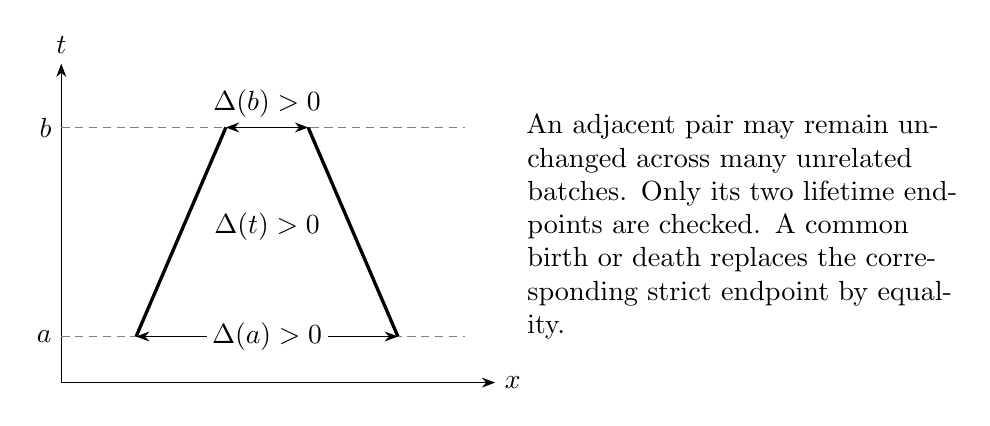
\begin{tikzpicture}[x=0.95cm,y=0.9cm,>=Stealth]
 \draw[->] (0,0)--(5.8,0) node[right] {$x$};
 \draw[->] (0,0)--(0,4.5) node[above] {$t$};
 \draw[densely dashed,gray] (0,0.65)--(5.4,0.65);
 \draw[densely dashed,gray] (0,3.6)--(5.4,3.6);
 \draw[very thick] (1,0.65)--(2.2,3.6);
 \draw[very thick] (4.5,0.65)--(3.3,3.6);
 \draw[<->] (1,0.65)--(4.5,0.65);
 \draw[<->] (2.2,3.6)--(3.3,3.6);
 \node[fill=white,inner sep=2pt] at (2.75,0.65) {$\Delta(a)>0$};
 \node[above] at (2.75,3.6) {$\Delta(b)>0$};
 \node[left] at (0,0.65) {$a$};
 \node[left] at (0,3.6) {$b$};
 \node at (2.75,2.2) {$\Delta(t)>0$};
 \node[right,align=left,text width=5.4cm] at (6.1,2.2)
 {An adjacent pair may remain unchanged across many unrelated batches.
 Only its two lifetime endpoints are checked. A common birth or death
 replaces the corresponding strict endpoint by equality.};
\end{tikzpicture}
\caption{The affine gap between adjacent straight segments cannot become
zero in the interior if its permitted endpoint conditions hold.}
\label{fig:endpoints}
\end{figure}

\subsection{Soundness and completeness}

\begin{theorem}[Exact chronological chamber]
\label{thm:chamber}
Fix a rational signal machine, an initial label word, and a finite skeleton
$\sigma$. There is an effective construction of rational homogeneous linear
equalities and strict inequalities whose solution set is exactly the set of
real seed geometries realizing $\sigma$. All simultaneous collisions and all
extra incoming signals are accounted for. Every nonempty solution set is a
relatively open rational polyhedral cone in the kernel of its equality
matrix.
\end{theorem}
\begin{proof}
First reject malformed identities, overlapping or noncontiguous input
blocks, undefined rules under the nontransparent convention, and incoming
blocks whose velocities fail to decrease strictly from left to right.
The latter condition is necessary because immediately before a multiple
meeting, two incoming lines $s,r$ ordered left to right have gap
$(v_s-v_r)(t_e-t)>0$ and hence $v_s>v_r$.

Propagate every intercept and event coordinate using
\eqref{eq:meet}--\eqref{eq:out}. Add the additional incoming-incidence
equalities, equal-time conditions within each batch,
\eqref{eq:batchorder}, initial gap positivity, and all adjacency-interval
endpoint conditions described above. Every resulting expression is a
homogeneous rational linear form in $g$.

For soundness, suppose all these conditions hold. On each positive-duration
adjacency interval, the endpoint lemma gives strict separation in its
interior. Hence no adjacent pair meets at an unlisted intermediate time.
A meeting of nonadjacent signals would force an adjacent meeting: at the
first failure of strict spatial order, at least one consecutive gap is zero.
Thus no collision of any arity can occur between the listed batches.

At a batch boundary, the incidence equalities put the signals of each
specified block at its reconstructed common site. Every adjacent gap not
belonging to that block is strictly positive there. Consequently no additional
incoming signal can join the site. The same strict conditions separate the
sites of distinct blocks. They also exclude an omitted disjoint collision
elsewhere in the configuration: an omitted site would have a zero gap at a
boundary where strict positivity is imposed, or would lie in the interior of
an unchanged adjacency interval, where positivity has just been proved.

The deterministic rule is therefore applicable to exactly the listed
incoming set at each site. Its outgoing order is increasing in velocity,
so outputs separate in the right-hand time limit. Static identity validation
ensures that every segment has a legitimate birth and is consumed at most
once. Induction on batches now proves that the reconstructed execution is
exactly the actual initial prefix.

For completeness, consider an actual execution realizing $\sigma$. The
coordinate propagation agrees with its genuine intersection coordinates.
The extra incidences and batch-time equalities hold, batch times strictly
increase, and each endpoint gap is zero precisely at a common birth or
common death of the pair. Every other endpoint gap is positive. A pair of
straight segments with a common birth and a later common death cannot occur.
Thus the execution satisfies every generated condition.

Finally, a finite intersection of homogeneous equality subspaces and open
linear half-spaces is a relatively open convex cone in that subspace. If
nonempty, its strict inequalities leave a neighborhood in the equality
subspace around each point. All coefficients are rational.
\end{proof}

\subsection{The event-sparse bound}

\begin{theorem}[Linear number of chronology conditions]
\label{thm:rows}
Let $J$ be the number of positive-duration maximal adjacency intervals used
by the construction. Then
\begin{align}
 J&\le (n-1)+\sum_{e=1}^E(q_e+1)
       \le (n-1)+(m+1)E,\label{eq:Jbound}\\
 R_\sigma&\le 3(n-1)+(3m+1)E.\label{eq:Rbound}
\end{align}
These bounds apply before deduplication or removal of identically zero
equalities.
\end{theorem}
\begin{proof}
Initially there are $n-1$ adjacent pairs. Replacing a collision block by $q_e$
outputs creates at most $q_e-1$ internal output pairs and two external pairs,
for a total at most $q_e+1$ when $q_e\ge1$. If $q_e=0$, it creates at most one
bridge pair between the surviving neighbors. At a boundary or when neighboring
blocks change simultaneously, fewer pairs may be created. Existing unchanged
pairs need no new interval. This proves \eqref{eq:Jbound}.

There are $d=n-1$ initial gap inequalities, $B$ positive batch-time
increments, $\sum_e(p_e-2)$ additional incoming-incidence equalities,
$E-B$ equalities synchronizing the sites within batches, and $2J$ endpoint
conditions. Therefore
\begin{align*}
 R_\sigma
 &\le d+B+\sum_e(p_e-2)+(E-B)+2J\\
 &=d+\sum_ep_e-E+2J\\
 &\le d+(m-1)E+2d+2(m+1)E\\
 &=3d+(3m+1)E.
\end{align*}
\end{proof}

The word \emph{sparse} here refers to the number of geometric conditions,
not to the number of nonzero coefficients in each eliminated linear form.
A deeply propagated intercept may depend on every initial gap. Storing all
rows densely can take $O(dR_\sigma)$ coefficient slots; compiling them may
have additional bookkeeping cost. Neither \eqref{eq:Rbound} nor degree two
is a constant arithmetic-operation bound for an unbounded computation.

An implementation may scan the live list at each batch for simplicity.
That does not change the mathematical row bound. A linked-list implementation
can update adjacencies locally, while the attached small implementation
prioritizes clarity and exact arithmetic over this engineering optimization.

\section{Quadratic Diophantine certificates with unique slacks}
\label{sec:quadratic}

\subsection{Positive denominator clearing}

Every nonzero rational row can be multiplied by a positive common denominator
and then divided by the positive greatest common divisor of its integer
coefficients. For equality rows the sign may subsequently be normalized;
for strict inequality rows it may not. Negating a strict row would reverse
its meaning.

Delete identically zero equality rows. An identically zero strict row makes
the chamber empty. Remove duplicate rows of the same kind. Denote the
resulting integer matrices by $\mathsf E$ and $\mathsf G$, with $r$ equality
rows and $s$ strict rows. Their matrix presentation is a complete, explicit
description of the polynomial, even when its expanded quadratic has many
monomials.

\begin{theorem}[Unique-slack quadratic representation]
\label{thm:quadratic}
For a nonrejected skeleton, define
\begin{equation}
 P(g,z)=\|\mathsf E g\|_2^2+
        \|\mathsf Gg-\mathbf1-z\|_2^2,
 \qquad (g,z)\in\N^{d+s}.
 \label{eq:P}
\end{equation}
Then $P$ is an integer polynomial of total degree at most two, globally
nonnegative and convex on $\R^{d+s}$. Moreover,
\begin{equation}
 \exists z\in\N^s\ P(g,z)=0
 \quad\Longleftrightarrow\quad
 g\in\Z^d\cap\Ccal_\sigma.
 \label{eq:bijective}
\end{equation}
For every accepted $g$, the auxiliary tuple is unique:
\begin{equation}
 z=\mathsf Gg-\mathbf1.
 \label{eq:uniqueslack}
\end{equation}
\end{theorem}
\begin{proof}
Each summand is the square of an affine linear form with integer
coefficients. Thus $P$ is a quadratic sum of squares and has Hessian
$2A^{\mathsf T}A\succeq0$, where $A$ is the combined coefficient matrix of
these affine forms. Over the reals, and hence over the integers, a sum of
squares vanishes precisely when every squared form vanishes. Its zeros
therefore require $\mathsf E g=0$ and
$\mathsf G_jg=1+z_j\ge1$ for every strict row. Because these expressions are
integers, this is equivalent to $\mathsf Gg>0$. The chamber theorem proves
\eqref{eq:bijective}. The same equations force \eqref{eq:uniqueslack}, which
is a nonnegative integer tuple whenever $g$ is accepted.
\end{proof}

All event coordinates are reconstructed from $g$ and are absent from the
auxiliary tuple. This avoids arbitrary rational encodings with multiple
numerator--denominator representatives. If the seed itself is given as a
rational geometry in a different interface, one must separately choose and
validate an encoding or a scale; the uniqueness theorem should not be
silently transferred to a noncanonical rational encoding.

\subsection{What uniqueness does not assert}

The polynomial depends on the externally supplied skeleton. Its number of
rows and slack variables is not fixed independently of the requested
history. Even though each member of this family has unique auxiliary
witnesses, placing an arbitrary unbounded skeleton inside one fixed
Diophantine equation is a different task. An unspecified application of
MRDP to a skeleton verifier does not preserve this uniqueness for free.

The present result is therefore not a proof that all computably enumerable
sets admit single-fold or finite-fold Diophantine representations. Its
stronger-than-usual feature is narrower and fully explicit: for each fixed
collision skeleton, projection of \emph{all} natural zeros of \eqref{eq:P}
onto the initial gaps is a bijection onto the actual integer realizations.
There are no additional zeros corresponding to incomplete local histories.

\section{Causal depth controls denominators and coefficient size}
\label{sec:depth}

\subsection{A denominator invariant}

Work in the integer-speed normalization of Section~\ref{sec:model}, and set
\begin{equation}
 V=\max\bigl(1,\max_{a\in M}|v(a)|\bigr),\qquad
 D=\lcm\{|v(a)-v(b)|:v(a)\ne v(b)\}.
 \label{eq:VD}
\end{equation}
The least common multiple of an empty set is taken as $1$; in that case no
collision is possible from a simple initial configuration.

Assign depth zero to initial segments. The depth of an event is one plus
the maximum depth of its incoming segments. Every output segment inherits
the depth of its birth event. This is causal depth, not the chronological
index of the batch.

\begin{theorem}[Causal denominator bound]
\label{thm:denominator}
At an event of depth $h$, each coefficient of its time and position forms
belongs to $D^{-h}\Z$. The same holds for every outgoing intercept. At an
integer seed, the event coordinates therefore have reduced denominators
dividing $D^h$.
\end{theorem}
\begin{proof}
Initial intercept coefficients are integral. Suppose an event has depth $h$.
Its incoming intercepts have denominators dividing powers of $D$ no larger
than $D^{h-1}$. Put them over the common denominator $D^{h-1}$. Formula
\eqref{eq:meet} divides their difference by a nonzero integer velocity
difference dividing $D$. Its time coefficients thus belong to $D^{-h}\Z$.
The position and all output intercepts use only addition and multiplication
by integer velocities, preserving that lattice. Evaluation at integer gaps
preserves the same denominator divisibility.
\end{proof}

Only primes already present in the speed differences can appear in these
coordinate denominators at an integer seed. At a rational seed, primes in
its initial common denominator may also occur. Parallel collisions elsewhere
do not increase the denominator exponent along an unrelated causal chain.

This is an upper bound, not an assertion that all factors of $D^h$ occur.
Cancellations and special velocity configurations can make the actual
precision requirement much smaller. Section~\ref{sec:clock} exhibits an
explicit case in which exponential denominator magnitude is nevertheless
unavoidable.

\subsection{An explicit coefficient bound}

For a rational linear form, use the $\ell^1$ norm of its coefficient vector.
Put $K=2+4V$. Initial intercepts have norm at most $d$.

\begin{lemma}[Growth of propagated forms]
\label{lem:norm}
Every intercept of depth at most $h$ has coefficient norm at most $dK^h$.
Every event time and event position of depth at most $h$ satisfies the same
bound.
\end{lemma}
\begin{proof}
Assume the input intercept norms at a depth-$h$ event are at most
$M=dK^{h-1}$. A nonzero integer speed difference has absolute value at least
one, so \eqref{eq:meet} gives $\|t_e\|_1\le2M$. Consequently
\[
 \|x_e\|_1\le(1+2V)M,\qquad
 \|b_{\mathrm{out}}\|_1\le(1+4V)M.
\]
Each factor is at most $K$. Induction proves the claim; forms of smaller
depth obey the larger bound as well.
\end{proof}

\begin{proposition}[Integer row height]
\label{prop:height}
If the maximum event depth is $h$, each primitive integer chamber row can
be chosen with every coefficient of absolute value at most
\begin{equation}
 A=2d(1+V)(DK)^h.
 \label{eq:A}
\end{equation}
In particular, for a fixed machine, row coefficient bit lengths are
$O(h+\log d)$.
\end{proposition}
\begin{proof}
An endpoint gap is a difference of two intercepts plus a velocity difference
times a batch time. Its coefficient norm is at most
$2dK^h+2VdK^h=2d(1+V)K^h$. Additional incidence residuals and differences of
event times satisfy the same bound. Initial gap rows also do.
All these coefficients have denominators dividing $D^h$ by
Theorem~\ref{thm:denominator}. Multiplication by $D^h$ bounds every resulting
integer coefficient by \eqref{eq:A}. Passing to a primitive integer row can
only decrease this bound.
\end{proof}

The exponent in \eqref{eq:A} bounds coefficient \emph{magnitude}; its
logarithm is linear in depth. Exact rational arithmetic can therefore remain
polynomial in the externally bounded history length even when ordinary
fixed-precision floating-point simulation becomes unreliable. This is not
an assertion that the total number of events before acceptance has a
computable bound in the initial input length.

\section{Small integral realizations and finite-horizon synthesis}
\label{sec:small}

\begin{theorem}[Small positive integer seed]
\label{thm:small}
Let $\Ccal=\{g\in\R^d:\mathsf E g=0,\mathsf Gg>0\}$ be a nonempty chamber
whose strict rows include $g_i>0$. Suppose all matrix coefficients are
integers of absolute value at most $A\ge1$. Then $\Ccal$ contains a positive
integer point satisfying
\begin{equation}
 \max_i g_i\le d^{d/2}A^d.
 \label{eq:small}
\end{equation}
Thus every realizable collision skeleton has a realization with a seed
encoding of polynomial bit length in the explicit skeleton and initial
label word, for a fixed machine.
\end{theorem}
\begin{proof}
Homogeneity permits a positive scaling of any point in $\Ccal$ so that every
strict expression is at least $1$. Hence the closed rational polyhedron
\[
 Q=\{g:\mathsf E g=0,\mathsf Gg\ge\mathbf1\}
\]
is nonempty. It lies in $[1,\infty)^d$. Minimizing $\sum_i g_i$ over $Q$
attains an optimum: intersecting with a nonempty objective sublevel gives
a compact set. The optimal face is a nonempty compact polytope and has a
vertex; that point is also a vertex of $Q$.

At such a vertex choose $d$ independent active constraints, including
sufficient equality rows. They give a nonsingular integer matrix $B$ and a
right-hand side $c$ with entries in $\{0,1\}$. The vertex is $B^{-1}c$.
Let $\delta=|\det B|$, a positive integer. Cramer's rule shows that
$g=\delta B^{-1}c$ is integral. It is positive, satisfies the homogeneous
equalities, and has every strict row at least $\delta\ge1$.

Each coordinate of $g$ is, up to sign, a determinant in which one column of
$B$ has been replaced by $c$. Hadamard's inequality bounds its magnitude by
$d^{d/2}A^d$; using the sharper bound on the replaced column is unnecessary.
This proves \eqref{eq:small}. Combining it with \eqref{eq:A} gives the stated
bit-length conclusion.
\end{proof}

\begin{corollary}[Real, rational, and integer realizability coincide]
A fixed skeleton is realizable by a positive real seed if and only if it is
realizable by a positive rational seed, if and only if it is realizable by a
positive integer seed. Realizability is decidable by rational linear
feasibility, using $\mathsf E g=0,\mathsf Gg\ge\mathbf1$.
\end{corollary}

The equivalence is specific to homogeneous rational chambers. It should not
be transferred to arbitrary nonlinear geometry. Nor does the scaled integer
seed necessarily satisfy extra nonhomogeneous requirements such as an
absolute prescribed distance or a fixed deadline.

\begin{corollary}[An NP upper bound for bounded synthesis]
\label{cor:NP}
Fix a rational signal machine and a distinguished output label. Given an
initial label word of length $n$ and a unary bound $T$, the problem of whether
some positive seed produces the distinguished label within a complete prefix
containing at most $T$ collision sites is in NP.
\end{corollary}
\begin{proof}
A skeleton of at most $T$ sites has at most $T$ batches and at most $n+mT$
created signal identities. Since $m$ is fixed, its discrete description has
polynomial length in $n+T$. Guess such a skeleton, check its identities and
rules, and check that the distinguished label appears in its prefix.

If it is realizable, Theorem~\ref{thm:small} supplies a positive integer seed
with polynomial bit length: $d=n-1$, $h\le T$, and
$\log A=O(T+\log n)$ for the fixed machine. Guess that seed as well.
Propagating rational forms and verifying every chamber row then takes a
polynomial number of operations on polynomial-length integers. This is a
polynomial-time verifier. No search over exponentially long real numbers is
required.
\end{proof}

Only an upper bound is claimed. There is no NP-hardness result here. The
budget counts total sites, including all sites in the accepting batch, not
elapsed physical time. A physical-time bound can contain arbitrarily many
events and even an accumulation, so it is not interchangeable with $T$.

\section{Robustness and the rank of synchronization constraints}
\label{sec:robust}

The chamber description distinguishes two different sources of numerical
difficulty. A trace can be sensitive because it demands an exact equality
among initial gaps, or its exact coordinates can require large denominators
even while its combinatorial pattern is robust. The latter phenomenon will
occur in the accumulating clock.

\begin{theorem}[Certified perturbation radius and codimension]
\label{thm:robust}
Let $\Ccal=\{g:\mathsf E g=0,\mathsf Gg>0\}$ be nonempty, with zero strict
rows removed, and let $g^*\in\Ccal$. Define
\begin{equation}
 \rho(g^*)=\min_j\frac{\mathsf G_jg^*}{\|\mathsf G_j\|_1}>0.
 \label{eq:rho}
\end{equation}
Every perturbation $\eta\in\ker\mathsf E$ with
$\|\eta\|_\infty<\rho(g^*)$ preserves the skeleton. The chamber has relative
dimension $d-\rank\mathsf E$. It has nonempty ambient interior if and only
if $\rank\mathsf E=0$; otherwise it has ambient Lebesgue measure zero.
\end{theorem}
\begin{proof}
The equality constraints persist for $\eta\in\ker\mathsf E$. For every
strict row, H\"older's elementary norm inequality gives
\[
 \mathsf G_j(g^*+\eta)
 \ge \mathsf G_jg^*-\|\mathsf G_j\|_1\|\eta\|_\infty>0.
\]
Hence the perturbed point stays in the chamber. This proves relative
openness in the full equality kernel, whose dimension is
$d-\rank\mathsf E$. A proper linear subspace has empty interior and measure
zero in $\R^d$. Conversely, when the rank is zero, the finitely many strict
inequalities define an open neighborhood of each accepted point.
\end{proof}

The radius in \eqref{eq:rho} is a certified lower bound, not necessarily the
largest possible radius in the equality subspace. Restricting perturbations
to that subspace can increase the true distance to a forbidden boundary.

One must also distinguish genuinely independent synchronization equations
from identities already forced by previous dynamics. Some formal
coincidences yield an identically zero row and impose no additional
codimension. Therefore the statement ``every multiple collision is fragile''
is too strong. What matters is the rank of the \emph{nontrivial} conditions
on the input geometry. When a loader or problem specification already
restricts the admissible inputs to a subspace, robustness should be measured
relative to that allowed input space.

The theorem provides a useful diagnostic for a proposed geometric computer.
A simulator can report not merely a diagram, but also an exact equality
matrix, a synchronization rank, and a rational certified tolerance at an
integer seed. Those objects separate an intended robust mechanism from an
accidental coincidence created by a particular numeric sample.

\section{Finite-horizon acceptance, semilinearity, and counting}
\label{sec:counting}

\subsection{Disjoint first-acceptance chambers}

Fix a machine, an initial label word, a marked accepting label, and a site
budget $T$. Acceptance means the first appearance of that label in a batch
such that the total number of processed sites through that entire batch is
at most $T$. If the initial word already contains the marked label, every
seed accepts with zero events.

There are only finitely many candidate skeletons with at most $T$ sites.
Indeed, at every stage there are at most $n+mT$ identities; the rule table
and possible contiguous input blocks are finite. Enumerate those skeletons
that end at the first accepting batch and reject all statically invalid
ones. Distinct nonempty chambers in this first-acceptance list are disjoint:
for a fixed seed, deterministic complete chronology has just one first
accepting prefix.

\begin{theorem}[Finite-horizon semilinearity]
\label{thm:semilinear}
The positive integer seed geometries accepted within site budget $T$ form
an effectively constructible semilinear set. More specifically, they are a
finite disjoint union of the integer points of rational homogeneous
chambers of the form \eqref{eq:mainchamber}.
\end{theorem}
\begin{proof}
The enumeration above is finite and effective. For each skeleton,
Theorem~\ref{thm:chamber} gives a complete linear characterization. On integer
points, a strict integer inequality is equivalent to being at least $1$,
so each chamber is definable in Presburger arithmetic. Finite union remains
Presburger-definable. The effective equivalence with semilinear sets is the
classical theorem of Ginsburg and Spanier~\cite{ginsburgspanier}.
\end{proof}

This use of the classical equivalence is not a new proof of that theorem.
The new substrate-specific input to it is the exact finite union of
collision chambers, including chronology and simultaneous-event boundaries.

\subsection{A single quartic for an unknown bounded first-hit skeleton}

The skeleton need not remain externally supplied when the event budget is
fixed. Enumerate the nonrejected first-acceptance skeletons
$\sigma_1,\ldots,\sigma_K$ and let their matrices be
$\mathsf E_k,\mathsf G_k$. Empty chambers may remain in this list without
harm. Introduce natural selectors $b_1,\ldots,b_K$ and a separate slack
vector $z_k$ for each chamber. Define
\begin{align}
 Q_T(g,b,z)
  ={}&\left(\sum_{k=1}^K b_k-1\right)^2
  +\sum_{k=1}^K\sum_i\bigl(b_k\mathsf E_{k,i}g\bigr)^2\notag\\
  &+\sum_{k=1}^K\sum_j
       \bigl(b_k(\mathsf G_{k,j}g-1)-z_{k,j}\bigr)^2.
 \label{eq:quarticunion}
\end{align}
For an empty family, use $Q_T=1$.

\begin{theorem}[Canonical first-hit quartic]
\label{thm:quarticunion}
Equation \eqref{eq:quarticunion} is a globally nonnegative integer polynomial
of degree at most four. Its natural zeros project bijectively onto the
integer seeds accepted within the fixed event budget. No Boolean equations
for the selectors and no additional inactive-slack constraints are needed.
\end{theorem}
\begin{proof}
At a natural zero, $\sum_kb_k=1$ forces exactly one selector to be $1$ and
all others to be $0$. For the selected chamber, the remaining equations are
precisely $\mathsf E_kg=0$ and
$\mathsf G_kg-\mathbf1=z_k\ge0$. For an unselected chamber, each slack
residual becomes $-z_{k,j}$, forcing all of its slacks to zero. Thus the
polynomial accepts exactly the union of the chamber integer points.

Those chambers are disjoint by canonical first-acceptance chronology.
Therefore an accepted seed determines exactly one selected skeleton, its
active slacks are uniquely determined, and every inactive slack is zero.
Every residual has degree at most two before squaring, proving the quartic
bound. The construction is a sum of squares and hence globally nonnegative,
but it is not in general convex.
\end{proof}

The same construction works for any finite disjoint family of chambers. If
chambers overlap, it still represents their union, but a seed in several
chambers has several selector witnesses. First-hit canonicalization is
therefore mathematically important, not cosmetic.

This theorem removes external skeleton choice for a \emph{bounded} problem;
it does not remove the bound. The number of candidate skeletons, and hence
the number of selectors and slacks, may be very large and grows with $T$.
The attached implementation provides the matrix-based quartic constructor,
and checks a two-chamber first-hit example. It does not include an optimized
exhaustive enumerator for all skeletons of an arbitrary event budget.

\subsection{Exact quasi-polynomials rather than merely leading asymptotics}

Let $A_T(H)$ count the accepted seeds in $\{1,\ldots,H\}^d$, with $H\ge1$.
For a single chamber put
\[
 \Pi_\sigma=\Ccal_\sigma\cap(0,1]^d.
\]
Its closure is a bounded rational polytope in its equality subspace.
The original set is obtained from that closed polytope by excluding finitely
many rational faces where one or more required strict expressions vanish.
The upper box facets remain included.

\begin{theorem}[Exact finite-horizon counting]
\label{thm:ehrhart}
For fixed machine, initial word, accepting label, and event budget $T$,
$A_T(H)$ is an exact quasi-polynomial in $H$ for all positive integers $H$.
It has degree at most $d$. Its ordinary generating function is rational and
has poles only at roots of unity. Furthermore,
\begin{equation}
 \lim_{H\to\infty}\frac{A_T(H)}{H^d}
 =\sum_{\sigma}\vol_d(\Pi_\sigma)\in\Q,
 \label{eq:density}
\end{equation}
where the sum ranges over the first-acceptance chambers, and
lower-dimensional terms have zero $d$-dimensional volume.
\end{theorem}
\begin{proof}
Homogeneity gives
$\Ccal_\sigma\cap(0,H]^d=H\Pi_\sigma$.
For a nonempty chamber, the closure of $\Pi_\sigma$ is obtained by replacing
its strict homogeneous inequalities by weak ones. To see equality with this
weak closure, take a small strictly feasible point with every coordinate
less than $1$ and form convex combinations with any weakly feasible point.
Those combinations converge to the latter while preserving all strict
conditions and the box.

A forbidden equality $\mathsf G_jg=0$ cuts out a face of the weak closure,
since $\mathsf G_jg\ge0$ throughout it. Inclusion--exclusion over these faces
expresses the lattice-point count in $H\Pi_\sigma$ as a finite integer
combination of counts in dilates of closed rational polytopes. Ehrhart's
rational-polytope theorem makes each term a quasi-polynomial; see
Beck and Robins~\cite{beckrobins}. This also covers lower-dimensional faces.
Disjointness of first-acceptance chambers permits summing these exact counts.

A quasi-polynomial of degree at most $d$ and period $p$ has a rational
generating function whose denominator divides a power of $1-z^p$.
This proves the generating-function assertion. The normalized leading
coefficient of a full-dimensional rational polytope count is its volume;
removing proper faces does not change it. Equivalently, the same limit follows
from Riemann sums for a bounded polyhedral set. Rational polytopes have
rational volume by a rational triangulation and determinant formulas.
Summing over the disjoint chambers proves \eqref{eq:density}.
\end{proof}

Thus a finite-horizon seed-counting problem has a particularly rigid
asymptotic form: a polynomial in $H$ with periodic coefficient functions,
not an arbitrary irregular error term. Its leading density is rational.
If the initial gaps are instead sampled independently and uniformly from
$(0,1]$, the probability of finite-horizon acceptance is exactly the same
rational volume sum.

The theorem does not promise an efficient procedure for enumerating all
chambers or computing all their volumes. Their number can grow rapidly with
$T$. It also does not justify interchanging an unbounded-time limit with the
box-size limit. Removing the event bound can leave an infinite union of
chambers, outside the finite quasi-polynomial argument.

Because each integer seed in one chamber has one slack tuple, its chamber
count is also the number of complete natural zeros of its quadratic
certificate with $1\le g_i\le H$, even when no separate bound is placed on
$z$. Across different skeletons this statement uses a tagged disjoint family
of certificates, not a single unqualified polynomial.

\section{An exact first-collision tournament}
\label{sec:tournament}

\subsection{Three chambers and a complete polynomial}

Consider labels $A,B,C$ with respective speeds $2,0,-1$, initially at
$0,u,u+v$, where $u,v>0$. Introduce two stationary output labels $H,R$ and
rules
\[
 \{A,B\}\longrightarrow\{H\},\qquad
 \{B,C\}\longrightarrow\{R\},\qquad
 \{A,B,C\}\longrightarrow\{R\}.
\]
Use transparent rules otherwise. The question here is whether $H$ is
produced at the \emph{first} collision batch.

The possible first events are exactly
\begin{equation}
 \begin{array}{c|c|c}
 \text{event}&\text{condition}&\text{time}\\\hline
 AB&u<2v&u/2\\
 BC&u>2v&v\\
 ABC&u=2v&v=u/2.
 \end{array}
 \label{eq:tournament}
\end{equation}
For instance, the formal $AC$ meeting time is $(u+v)/3$. If $u<2v$, it is
later than $u/2$; if $u>2v$, it is later than $v$. It cannot be a different
first event. The equality case is the triple collision.

The complete accepting chamber has the particularly small certificate
\begin{equation}
 P_{AB}(u,v,z_1,z_2,z_3)=
 (u-1-z_1)^2+(v-1-z_2)^2+(2v-u-1-z_3)^2.
 \label{eq:tournamentpoly}
\end{equation}
All five variables range over $\N$. At $u=v=1$, for example, the unique
auxiliary tuple is $(0,0,0)$. At $(u,v)=(3,1)$, the third strict condition
fails, correctly rejecting the incidence-only counterfeit. At $(2,1)$ it
also fails, correctly rejecting an omitted simultaneous third input.

For the triple-collision skeleton the compiler instead produces
\begin{equation}
 P_{ABC}(u,v,z_1,z_2)=
 (u-2v)^2+(u-1-z_1)^2+(v-1-z_2)^2.
 \label{eq:triplepoly}
\end{equation}
Its equality rank is one. The two binary-event chambers have rank zero and
are open in the positive quadrant; the triple-collision chamber is
one-dimensional and requires exact synchronization.

\begin{figure}[htbp]
\centering
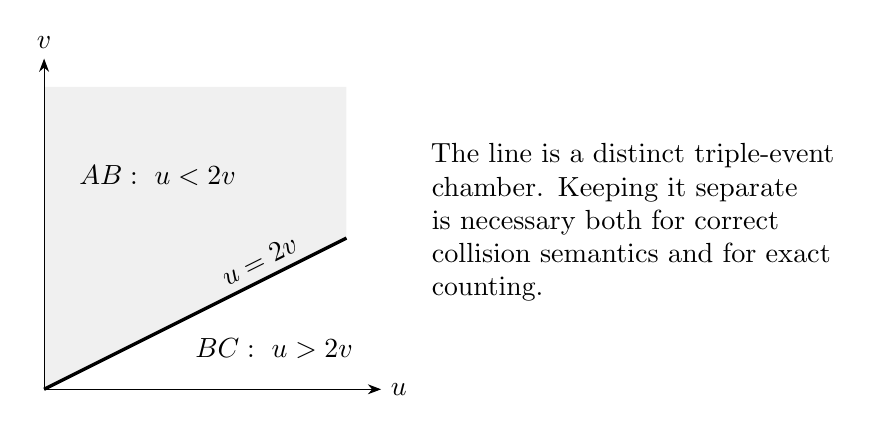
\begin{tikzpicture}[x=0.8cm,y=0.8cm,>=Stealth]
 \fill[gray!12] (0,0)--(4.8,2.4)--(4.8,4.8)--(0,4.8)--cycle;
 \draw[->] (0,0)--(5.35,0) node[right] {$u$};
 \draw[->] (0,0)--(0,5.25) node[above] {$v$};
 \draw[very thick] (0,0)--(4.8,2.4);
 \node[rotate=26.565,above] at (3.55,1.78) {$u=2v$};
 \node at (1.8,3.4) {$AB:\ u<2v$};
 \node at (3.65,0.65) {$BC:\ u>2v$};
 \node[right,align=left,text width=5.1cm] at (6,2.65)
 {The line is a distinct triple-event chamber. Keeping it separate is
 necessary both for correct collision semantics and for exact counting.};
\end{tikzpicture}
\caption{The first-event geometry is partitioned into two open cones and a
synchronization ray. The coordinate axes are excluded.}
\label{fig:chambers}
\end{figure}

\subsection{Counting, generating function, and inversion}

Let $C(H)$ count the accepting gap pairs with $1\le u,v\le H$, and set
$C(0)=0$. Direct summation gives
\begin{align}
 C(H)&=\sum_{v=1}^H\min(H,2v-1)\notag\\
 &=\begin{cases}
 3m^2,&H=2m,\\
 3m^2+3m+1,&H=2m+1,
 \end{cases}\notag\\
 &=\floor{\frac{3H^2+1}{4}}
  =\frac{3H^2}{4}+\frac{1-(-1)^H}{8}.
 \label{eq:count}
\end{align}
For $H=2m$, split the sum after $v=m$; the odd-number sum contributes $m^2$
and the remaining $m$ terms contribute $2m^2$. The odd case follows by the
same split after $m+1$.

The first values are
\[
 0,1,3,7,12,19,27,37,48,61,75,91,108,127,147,169,\ldots.
\]
No assertion about an OEIS identification or novelty of this elementary
sequence is needed. It is included as an exactly solvable counting test for
the compiler and as an illustration of the general quasi-polynomial theorem.
Its ordinary generating function is
\begin{equation}
 \sum_{H\ge0}C(H)z^H
 =\frac{z(1+z+z^2)}{(1-z)^3(1+z)}.
 \label{eq:gf}
\end{equation}
This follows from the standard geometric-series derivatives applied to
\eqref{eq:count}, or by expanding the displayed rational function.

There is also an exact inverse threshold. For every positive integer $y$,
\begin{equation}
 \min\{H\ge0:C(H)\ge y\}
 =\ceil{\sqrt{\frac{4y-1}{3}}}.
 \label{eq:inverse}
\end{equation}
Indeed, because $y$ is integral,
$\floor{(3H^2+1)/4}\ge y$ is equivalent to $3H^2+1\ge4y$.
The smooth expression inside the ceiling has the expansion
\begin{align}
 \sqrt{\frac{4y-1}{3}}
 &=\frac{2}{\sqrt3}y^{1/2}
 -\frac{1}{4\sqrt3}y^{-1/2}
 -\frac{1}{64\sqrt3}y^{-3/2}
 -\frac{1}{512\sqrt3}y^{-5/2}
 +O(y^{-7/2}).
 \label{eq:inverseasymptotic}
\end{align}
The binomial series supplies all further orders. The ceiling in
\eqref{eq:inverse} is essential: omitting it would incorrectly replace an
integer inverse's bounded rounding oscillation by a decaying error.

\subsection{Independent simultaneous sites}

Take the transparent two-speed machine with $v(P)=1$, $v(N)=-1$, and initial
word $P,N,P,N$. With gaps $(2,5,2)$, the two disjoint pairs $(0,1)$ and
$(2,3)$ collide simultaneously at time $1$. A correct first batch must
contain both sites. A proposed batch containing only $(0,1)$ is rejected by
the unchanged adjacency interval of $(2,3)$, whose gap would vanish at the
final boundary where positivity is required.

For general positive gaps $(g_1,g_2,g_3)$, this simultaneous first-batch
skeleton has the single nontrivial equality $g_1=g_3$. Changing the last gap
from $2$ to $3$ destroys that equality. This example tests a different
failure mode from the omitted third input of a multiple collision: the
missing event is spatially separate, not an extra signal at the same site.

\section{A four-speed clock with exponentially growing denominators}
\label{sec:clock}

\subsection{Rules and a closed-form execution}

Consider the four labels
\[
 v(L)=0,\qquad v(P)=2,\qquad v(R)=-1,\qquad v(N)=-2
\]
with rules
\begin{equation}
 \{P,R\}\longrightarrow\{N,R\},\qquad
 \{L,N\}\longrightarrow\{L,P\},
 \label{eq:clockrules}
\end{equation}
and transparent defaults. Initially put $L$ at $0$, $P$ at $u$, and $R$ at
$u+v$, with $u,v>0$. The left boundary is stationary, the right boundary
moves left at speed $1$, and a particle alternately travels right at speed
$2$ and left at speed $2$, reflecting at the boundaries via the two rules.

Write $S=u+v$ and $W=3u+2v$. The collision times are
\begin{align}
 t_{2k+1}&=S-\frac{W}{3^{k+1}},&&k\ge0,\label{eq:clockodd}\\
 t_{2k}&=S-\frac{W}{2\cdot3^k},&&k\ge1.\label{eq:clockeven}
\end{align}
Odd collisions occur on the right boundary at position $S-t_{2k+1}$;
even collisions occur at position zero.

\begin{proposition}[Clock correctness and common chamber]
\label{prop:clock}
For every $u,v>0$, equations \eqref{eq:clockodd}--\eqref{eq:clockeven}
describe the actual alternating execution. The collision times strictly
increase to $S$. Every finite alternating prefix has the whole positive
$(u,v)$ quadrant as its seed chamber.
\end{proposition}
\begin{proof}
The first rightward meeting occurs at $t_1=v/3$, which equals
$S-W/3$. At a right-boundary collision at time $t$, the remaining boundary
distance is $S-t$. The new left-moving particle takes $(S-t)/2$ to reach
zero, leaving time-to-boundary-meeting $(S-t)/2$. From there the right-moving
particle closes the remaining gap at relative speed $3$, leaving two thirds
of that remaining time when it next hits the right boundary. Hence a full
right-to-right bounce multiplies $S-t$ by $1/3$, with the intermediate
left collision having half the previous remaining time. This proves the
formulas inductively.

The first time is positive. Every subsequent difference is positive, and
all times are less than $S$. Between collisions the moving particle lies
strictly between the two boundaries. The boundaries themselves meet only at
$S$, not at any finite indexed event. There is therefore no unlisted
collision in any finite prefix. The labels alternate exactly as specified
by \eqref{eq:clockrules}, independently of the positive gaps. This proves
both correctness and the common-chamber statement.
\end{proof}

\begin{figure}[htbp]
\centering
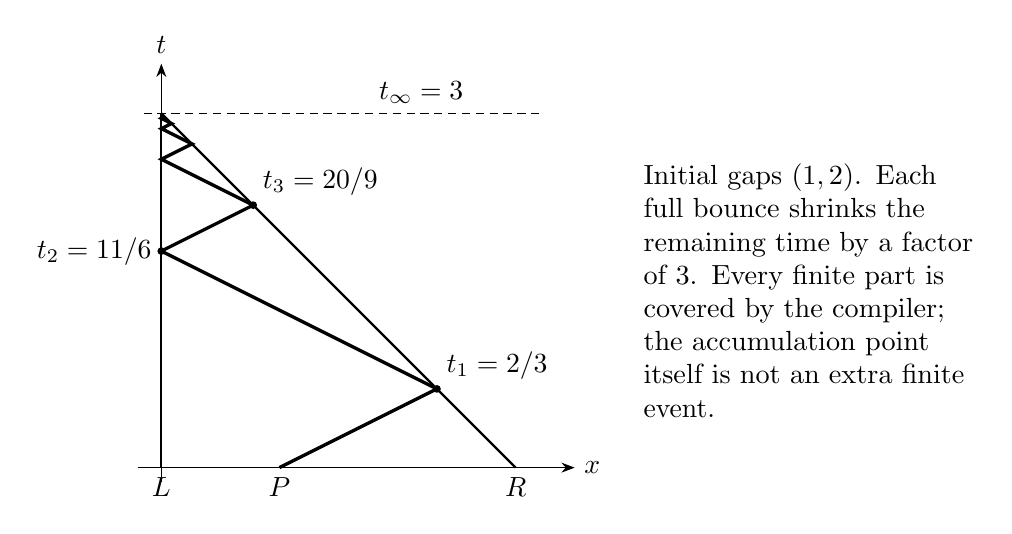
\begin{tikzpicture}[x=1.5cm,y=1.5cm,>=Stealth]
 \draw[->] (-0.2,0)--(3.5,0) node[right] {$x$};
 \draw[->] (0,-0.12)--(0,3.42) node[above] {$t$};
 \draw[thick] (0,0)--(0,3);
 \draw[thick] (3,0)--(0,3);
 \draw[densely dashed] (-0.15,3)--(3.2,3);
 \draw[very thick] (1,0)--(2.333333,0.666667)--(0,1.833333)
 --(0.777778,2.222222)--(0,2.611111)--(0.259259,2.740741)
 --(0,2.870370)--(0.086420,2.913580)--(0,2.956790)
 --(0.028807,2.971193);
 \fill (2.333333,0.666667) circle (1.4pt);
 \fill (0,1.833333) circle (1.4pt);
 \fill (0.777778,2.222222) circle (1.4pt);
 \node[below] at (0,0) {$L$};
 \node[below] at (1,0) {$P$};
 \node[below] at (3,0) {$R$};
 \node[above right] at (2.333333,0.666667) {$t_1=2/3$};
 \node[left] at (0,1.833333) {$t_2=11/6$};
 \node[above right] at (0.777778,2.222222) {$t_3=20/9$};
 \node[above] at (2.2,3) {$t_\infty=3$};
 \node[right,align=left,text width=4.2cm] at (4,1.5)
 {Initial gaps $(1,2)$. Each full bounce shrinks the remaining time by
 a factor of $3$. Every finite part is covered by the compiler;
 the accumulation point itself is not an extra finite event.};
\end{tikzpicture}
\caption{A four-speed accumulating clock. The drawing displays only a finite
number of segments; the formulas specify all finite prefixes.}
\label{fig:clock}
\end{figure}

\subsection{A denominator lower bound without fragile synchronization}

For the particular integer seed $(u,v)=(1,2)$, $S=3$ and $W=7$, giving
\[
 \frac23,\frac{11}6,\frac{20}9,\frac{47}{18},\frac{74}{27},
 \frac{155}{54},\frac{236}{81},\frac{479}{162},\ldots.
\]
At event $2k$, the reduced denominator is exactly $2\cdot3^k$:
\[
 t_{2k}=\frac{6\cdot3^k-7}{2\cdot3^k},
\]
and the numerator is odd and is not divisible by $3$. The causal depth of
event $j$ is $j$, since the reflected particle links every event to its
predecessor. Thus denominator magnitude is exponential in causal depth,
while its bit length is linear in depth.

Here the integer speed differences have least common multiple $D=12$,
so Theorem~\ref{thm:denominator} correctly gives a divisible upper bound
$12^j$. The example does not make that upper bound sharp in its base, but it
rules out a depth-independent denominator bound or a polynomial-magnitude
bound for general rational signal machines.

At the same time, every finite prefix has equality rank zero and remains
valid throughout the positive quadrant. Growing exact precision is therefore
not evidence of a fragile collision pattern. Robust symbolic chronology and
large rational denominators are compatible.

Accumulations in signal machines are established phenomena. Becker et
al.~\cite{accumulations} distinguish the behavior of small speed sets and
show, in particular, that four speeds permit accumulation whereas the
three-speed case with rational speed and initial-distance ratios does not.
The clock is an explicit test case and a denominator-growth illustration,
not a claim to have discovered accumulation. Our compiler verifies every
ordinary finite prefix before $S$; it assigns no transition or computational
power to the limiting point at $S$.

\section{Why a fixed universal convex quadratic cannot follow}
\label{sec:barrier}

A natural question is whether the quadratic frontend can be compressed into
one fixed polynomial with a fixed number of witnesses for arbitrary
unbounded computations. Within the globally nonnegative quadratic class,
there is an elementary obstruction stronger than a failure of the present
construction.

\begin{theorem}[Linear zero-set rigidity]
\label{thm:rigidity}
Let $Q(w)$ be a quadratic polynomial with rational coefficients that is
nonnegative for every $w\in\R^N$. Its real zero set is either empty or a
rational affine subspace. The projection of its nonnegative integer zeros
onto any subset of coordinates is an effectively semilinear, decidable set.
\end{theorem}
\begin{proof}
Write
\[
 Q(w)=w^{\mathsf T}Aw+2b^{\mathsf T}w+c
\]
with $A$ rational and symmetric. Global nonnegativity implies $A\succeq0$.
It also implies $b\perp\ker A$: otherwise the restriction to an appropriate
kernel direction would be a nonconstant affine function unbounded below.
Thus $b\in\operatorname{range} A$ and the consistent rational system
$Aw_0=-b$ has a rational solution.

Completing the square gives
\[
 Q(w)=(w-w_0)^{\mathsf T}A(w-w_0)+\mu,
 \qquad \mu=c+b^{\mathsf T}w_0\ge0.
\]
If $\mu>0$, there are no zeros. If $\mu=0$, positive semidefiniteness gives
$Q(w)=0$ exactly when $A(w-w_0)=0$, equivalently $Aw=-b$. This is a rational
affine subspace.

Clearing denominators gives finitely many integer linear equations.
Intersecting with $\N^N$ and projecting coordinates is an existential
Presburger definition. Effective semilinearity and decidability follow from
Ginsburg--Spanier and Presburger arithmetic~\cite{ginsburgspanier}.
\end{proof}

\begin{corollary}[Convex-quadratic compression barrier]
\label{cor:barrier}
An undecidable halting relation cannot be represented by one fixed globally
nonnegative rational quadratic with a fixed finite number of natural
parameters and witnesses, even after a computable input-loading map.
\end{corollary}
\begin{proof}
The projected zero relation would be decidable by
Theorem~\ref{thm:rigidity}. Its preimage under a computable input-loading map
would then be decidable as well, contradicting the assumed undecidability.
\end{proof}

This theorem applies to global nonnegativity on \emph{all real variables},
not merely nonnegativity on a special natural-number input slice. It does
not classify arbitrary quadratic equations, arbitrary nonconvex
polynomials, or cubic Diophantine representations. For example,
$x-y^2=0$ is a quadratic equation with a nonlinear zero set, but its
polynomial is not globally nonnegative and is outside the theorem.

The quartic first-hit construction in \eqref{eq:quarticunion} leaves the
convex-quadratic class by multiplying selectors and input-dependent linear
forms. Its finite-horizon relation remains decidable for other reasons.
A truly unbounded compiler must additionally encode an unbounded amount of
discrete chronology into finitely many integer variables. That compression,
not the local collision geometry, is where the universal Diophantine
problem re-enters.

\subsection{The classical unbounded existence result remains available}

For a finite rational initial configuration, an exact event-driven simulator
can find the next collision batch by computing all positive pairwise meeting
times and taking the smallest. It can then apply all rules at the sites of
that batch. Repeating this procedure semidecides the appearance of a marked
signal in an ordinary finite prefix. An infinite accumulating run simply
causes the simulator to execute indefinitely when no earlier acceptance has
occurred; no post-accumulation convention is needed for semidecidability.

Consequently the pre-accumulation finite-prefix acceptance relation, with
machine and rational input encoded by natural numbers, is computably
enumerable. MRDP supplies a fixed-arity Diophantine representation of that
encoded relation~\cite{matiyasevich,afp}. This last existence step is
classical. Neither MRDP nor the present frontend automatically supplies
unique witnesses, an explicit small expanded universal polynomial, or the
repository's particular operation ledger.

For a fixed universal machine with an undecidable marked-halting interface,
there can be no total computable function of the encoded seed that bounds
the number of sites needed by every accepting run. Such a function, followed
by exact bounded simulation, would decide halting. This explains why the
bounded chamber theorems and the universal existence theorem coexist without
contradiction.

\section{Implementation, reproducible checks, and trust boundaries}
\label{sec:implementation}

\subsection{What the attached code computes}

The accompanying standard-library Python implementation uses exact
\texttt{Fraction} arithmetic for every geometric calculation. The essential
interfaces are:
\begin{lstlisting}[language=Python]
Machine(speeds, rules, transparent_default=True)
simulate(machine, initial_labels, gaps, max_batches=20)
compile_skeleton(machine, initial_labels, skeleton)
UnionCertificate(tuple_of_chamber_certificates)
\end{lstlisting}
A skeleton is a tuple of batches; each batch is a tuple of input-ID tuples.
For example, \texttt{(((0, 1), (2, 3)),)} denotes one batch with two
independent simultaneous sites. Fresh identities are generated canonically
by increasing outgoing velocity.

The simulator uses an all-pairs minimum-time calculation. The symbolic
compiler uses intercept propagation and adjacency intervals. Their different
chronology mechanisms provide a useful cross-check: the regression suite
compares exact numerical prefixes against the regions predicted by the
symbolic compiler on many other initial seeds.

A compiled \texttt{Certificate} contains the complete integer matrices,
exact rational event forms, causal depths, interval count, and raw row
ledger. Its \texttt{witnesses(gaps)} method returns the unique natural slack
tuple, while \texttt{evaluate(gaps, witnesses)} evaluates the full polynomial.
The \texttt{UnionCertificate} implements \eqref{eq:quarticunion}. Its
constructor does not prove that a supplied family is globally disjoint;
that is a mathematical precondition for uniqueness. At a supplied seed,
its witness routine rejects multiple accepting chambers rather than
silently claiming a unique answer.

The machine constructor copies and freezes the speed and rule tables.
This prevents a caller's later dictionary mutation from changing the
meaning of an already constructed machine. Input validation rejects unknown
labels, repeated-speed outputs, malformed groups, use of dead signals,
noncontiguous blocks, overlapping sites, and inappropriate incoming speed
orders. These checks are part of the semantic contract.

The exported JSON matrices specify full polynomials, not just sample zeros.
For example, \texttt{tournament\_left.json} contains all rows of
\eqref{eq:tournamentpoly}, while
\texttt{first\_hit\_quartic\_union.json} supplies every matrix and the exact
selector formula for a two-chamber union. Expanding these expressions into
monomials is optional and provides no extra mathematical information.

\subsection{Run and reproduce}

From the extracted archive's root directory, run
\begin{lstlisting}[language=bash]
python code/run_checks.py
latexmk -pdf -interaction=nonstopmode -halt-on-error article.tex
\end{lstlisting}
Python 3.10 or newer and a standard LaTeX installation are sufficient.
No Python third-party dependencies are needed. The test command overwrites
the generated JSON data with deterministic results, including
\texttt{data/checks.json}.

The completed run accompanying this manuscript passed \textbf{34,560 exact
assertions}. Its principal coverage is summarized in
Table~\ref{tab:tests}. These are finite regression tests, not exhaustive
verification of all machines or all input geometries.

\begin{table}[htbp]
\centering
\small
\begin{tabular}{p{0.57\linewidth}r}
\toprule
Check family & Instances\\
\midrule
Tournament seeds $(u,v)\in\{1,\ldots,40\}^2$ & 1,600\\
Exact seed-count boxes $H=0,\ldots,80$ & 81\\
Exact inverse thresholds $y=1,\ldots,2000$ & 2,000\\
Four-speed clock batches at $(1,2)$ & 24\\
Other positive clock seeds with the same 24-batch skeleton & 25\\
Pseudorandom rule tables (fixed random seed 20261002) & 6\\
Distinct nonempty prefix skeletons obtained from those tables & 24\\
Independent seed--skeleton chronology comparisons & 1,536\\
Two-chamber quartic-union seed checks & 1,600\\
\bottomrule
\end{tabular}
\caption{Finite exact test coverage. Individual assertions also check
witness mutations, denominators, malformed inputs, and table immutability.}
\label{tab:tests}
\end{table}

The pseudorandom cases include creation, annihilation, and transparent rules.
The checked skeletons are generated from exact sample executions and then
tested against other seed geometries. The suite also specifically rejects
an earlier omitted collision, an omitted third input, and an omitted
independent simultaneous site. It tests the clock's exact closed-form times
and denominator divisibility. For the quartic union, it checks selector
validity and that inactive slacks are forced to zero.

\subsection{An auditable resource ledger}

Table~\ref{tab:ledger} separates retained conditions from raw generated rows.
The generic bound is deliberately loose; redundancy elimination can be
substantial. The 24-batch clock is a useful example: its entire seed chamber
reduces to only three retained strict rows, even though its geometric
coordinates become increasingly complicated. One of those rows is redundant
with positive gaps, but the implementation does not attempt full linear
redundancy minimization.

\begin{table}[htbp]
\centering
\small
\begin{tabular}{lrrrrrr}
\toprule
Certificate & $E$ & $B$ & $r$ & $s$ & Raw rows & Bound\\
\midrule
Tournament $AB$ & 1&1&0&3&7&16\\
Tournament $BC$ & 1&1&0&3&7&16\\
Tournament $ABC$ & 1&1&1&2&8&16\\
Two simultaneous sites & 2&1&1&4&11&23\\
Clock, 24 batches & 24&24&0&3&122&318\\
\bottomrule
\end{tabular}
\caption{Exact compiler ledger: $r$ is the retained equality count and $s$
the retained strict-row count. The rightmost column is
$3(n-1)+(3m+1)E$, not an arithmetic-operation count.}
\label{tab:ledger}
\end{table}

\subsection{What has and has not been verified}

The prose proofs establish general claims by mathematical argument. The
code and data test finite instances with exact arithmetic. No Lean or other
proof-assistant verification of this article is included, and the
implementation is not a formally verified compiler. The universal 13-type
machine's complete published rule table and finite-input loader have not
been reimplemented in the package. The code supplies a generic machine
interface and the specific worked examples only.

The repository was inspected on 2 October 2026. The observed main-branch
head was
\begin{center}\small\ttfamily
f1edb38f93aa0a362a34b531a600909f6e74608a.
\end{center}
The relevant reversible-history audit was fetched as blob
\begin{center}\small\ttfamily
cb31d0a108b9a19fc33da6fa89a73b604e15e260.
\end{center}
No repository-wide build was performed and no repository files were changed.
The current README and the older audit have different historical operation
ledgers; none is used as a theorem in the present proofs. The new row counts
are not comparable to a fixed-universal arithmetic count without a separate
input and history compression analysis.

\section{Further research questions and a concrete development path}
\label{sec:future}

\subsection{Formalizing the chronology theorem}

The most direct formalization target is the endpoint lemma followed by the
sweep invariant: the live list is in strict spatial order on every open
interval between batches, and its equal-position blocks at each boundary
are exactly the declared sites. Stable IDs make consumption and birth
finite-map properties. A Lean development should keep the real semantic
statement separate from rational coefficient computation, then prove that
evaluation commutes with the intercept compiler. Finally, the sum-of-squares
zero lemma and natural slack uniqueness can be linked to the repository's
Diophantine infrastructure.

A practical first milestone is a small checker for exported matrices and
rational event forms. A second is a proof-producing compiler rather than a
trusted Python translator. Tests that compare two unverified programs should
remain auxiliary evidence, not be promoted to kernel verification.

\subsection{An audited universal signal-machine frontend}

Instantiate a published finite-input universal construction with its exact
labels, velocities, all required collision rules, transparent defaults, input
encoding, and marked acceptance convention. The 13-type construction of
Durand-Lose~\cite{durandlose} is a concrete candidate. The task is not merely
to copy a picture: simultaneous three-input cases, finite workspace supply,
and the loader's correspondence with the simulated machine must be audited.
The eventual theorem should state an exact equivalence between an ordinary
integer program input and the existence of a compiled accepting prefix.

This would turn the present generic geometry theorem into a fully explicit
end-to-end substrate result. A fixed-arity universal polynomial would still
require a separate outer compression step and its own complete resource
ledger.

\subsection{Sharper denominator invariants}

The factor $D^h$ treats all speed differences uniformly. Can one use a
velocity-labelled dependency graph to compute exact prime-valuation bounds
or a smaller denominator ideal for each event? Which speed sets force
uniformly bounded denominators on all integral seeds, and which permit
exponential growth? The clock supplies one lower-bound mechanism, while the
small-speed accumulation results~\cite{accumulations} suggest that the
interaction between arithmetic precision and global dynamics is subtler
than a least-common-multiple bound alone.

A particularly concrete project is to propagate prime-valuation vectors
through \eqref{eq:meet} and detect systematic cancellation at each rule.
Any claimed lower bound must use reduced denominators, not merely the
unreduced fractions produced by a particular implementation.

\subsection{From few rows to small arithmetic circuits}

The event-sparse theorem controls row count but permits dense coefficient
vectors. Can common subexpressions in intercept forms give a substantially
smaller arithmetic circuit than dense matrix evaluation? An appropriate
cost model must distinguish fixed machine numerals, input-dependent
arithmetic, equality tests, and the conversion from a residual system to one
polynomial. The original intercept dependency graph already provides a
sharing structure; the challenge is to preserve its certified semantic
meaning while optimizing its arithmetic schedule.

A useful result would be a proved tradeoff among witness count, maximum
degree, coefficient height, and literal addition/multiplication count.
No one-dimensional comparison such as ``quadratic beats a degree-169
polynomial'' is meaningful when arity and unbounded-history coding differ.

\subsection{Avoiding exhaustive first-hit enumeration}

The quartic in \eqref{eq:quarticunion} is explicit but can contain an enormous
number of chambers. Can a local selector circuit encode a bounded unknown
skeleton with polynomially many variables while retaining canonical first-hit
uniqueness, including all simultaneous events? A promising direction is to
encode changes of adjacency directly rather than a rectangular array of all
particle positions. The main obstruction is that a locally plausible
selection must still describe one globally ordered and complete execution.

Even a polynomial-size bounded compiler would not solve fixed-arity
unbounded compression. Keeping those two improvements distinct will make
future operation claims interpretable.

\subsection{Robust universality and minimal synchronization rank}

For a given computational simulation, determine the rank of its required
input-geometry equalities. Can the same computation be realized on a
full-dimensional chamber, or does its interface genuinely require exact
ratios among certain gaps? The answer must be relative to the legal input
space rather than to coordinates the loader never permits to vary.

One possible invariant is the minimum independent synchronization rank
among equivalent signal-machine implementations with a fixed speed set.
The chamber theorem makes that invariant concrete for each finite trace,
but extending it uniformly over a universal family needs a precise notion
of simulation and allowed perturbation.

\subsection{Counting complexity and asymptotic structure}

Determine when first-hit chamber counts can be computed without enumerating
all skeletons. Are there useful machine classes for which a recurrence on
adjacency types produces the Ehrhart generating function directly? When do
quasi-polynomial periods collapse, and which restrictions imply polynomial
counts? The exact inverse in the tournament example is simple; in higher
degree, inverse asymptotics must retain residue-class corrections and
rounding effects rather than replacing them by an unjustified smooth error.

For unbounded acceptance, investigate convergence of finite-horizon rational
densities. The increasing accepted sets give monotonicity, but a rational
limit is not automatic. Quantitative tail estimates would be needed for a
useful approximation theorem and for interchanging input-box and time limits.

\subsection{Algebraic velocities and nonlinear motion}

With velocities in a fixed algebraic number field, formal event coordinates
remain linear over that field. However, positivity is no longer a rational
half-space condition in the same elementary form, and integer realization
by scaling is not automatic. A number-field sign certificate might extend
part of the method, but the rational-cone, Presburger, and Ehrhart conclusions
would require new arguments or additional hypotheses.

If signals accelerate or their velocities depend on variable parameters,
\eqref{eq:meet} ceases to divide only by a fixed constant. This identifies a
precise boundary of the present linearization. Studying which broader motion
laws still admit low-degree complete chronological certificates is a more
informative problem than assuming every geometric model behaves like the
fixed-speed case.

\subsection{Accumulation limits without fictitious infinite witnesses}

The clock gives a finitely described accumulation time, but a generic finite
prefix certificate cannot assert all events of an infinite run. A separate
notion of a certified self-similar tail could perhaps prove a limit formula
or a no-collision property beyond a given recursive pattern. Such a notion
must specify the dynamics and limit semantics explicitly. It must not
silently treat an infinite sequence of successful finite checks as one
ordinary existential Diophantine witness.

\section{Conclusion}

For rational fixed-speed signal machines, the continuous coordinates of a
finite computation are not the difficult nonlinear part. Once a discrete
chronological skeleton is fixed, they are rational linear forms in the
initial gaps. The nontrivial certificate obligation is completeness of
chronology: excluding unlisted earlier meetings and accounting for every
signal and every site at a simultaneous event. Maximal adjacency intervals
solve that obligation with a linear number of endpoint conditions.

The resulting exact chamber description yields quadratic natural-number
certificates with unique slack tuples, and finite disjoint first-hit unions
yield quartics with unique selector and slack tuples. It also yields useful
results about denominator growth, small integral realizations, perturbation
stability, and seed-counting quasi-polynomials. The executable examples test
these claims against independent exact simulation and expose the boundary
cases that incidence-only encodings miss.

The unresolved universal task is sharply separated: finitely encode an
unbounded discrete skeleton together with the ordinary input interface.
The convex-quadratic rigidity theorem explains why this cannot be achieved
by merely hiding more geometry inside one fixed globally nonnegative
quadratic. The present contribution is a complete and auditable geometric
frontend, together with a clear account of which further arithmetic and
formalization steps remain.

\appendix
\section{A minimal worked use of the compiler}
\label{app:example}

The following code can be run from the archive root. It builds the
first-collision tournament and constructs a complete certificate without
using an external algebra system.
\begin{lstlisting}[language=Python]
import sys
sys.path.insert(0, "code")
from signal_certificates import Machine, compile_skeleton

machine = Machine(
    {"A": 2, "B": 0, "C": -1, "H": 0, "R": 0},
    {
        frozenset(("A", "B")): ("H",),
        frozenset(("B", "C")): ("R",),
        frozenset(("A", "B", "C")): ("R",),
    },
)
skeleton = (((0, 1),),)
cert = compile_skeleton(machine, ("A", "B", "C"), skeleton)
gaps = (1, 1)
slacks = cert.witnesses(gaps)
assert cert.evaluate(gaps, slacks) == 0
assert not cert.accepts((3, 1))  # An earlier BC collision.
assert not cert.accepts((2, 1))  # A simultaneous ABC collision.
print(cert.to_dict())
\end{lstlisting}
The order of rows in the exported matrices is lexicographic and need not
match the order used in the displayed mathematical formula. Row order
changes only the order of slack coordinates, not the represented relation
or the uniqueness statement.

\section{Dependency map and claim status}

\begin{longtable}{>{\RaggedRight\arraybackslash}p{0.29\linewidth}>{\RaggedRight\arraybackslash}p{0.38\linewidth}>{\RaggedRight\arraybackslash}p{0.25\linewidth}}
\toprule
Claim & Principal ingredients & Status in this package\\
\midrule
\endhead
Exact chronology chamber & Intercept induction; affine endpoint lemma;
static identity and order validation & Full manuscript proof; exact tests\\
Event-sparse row bound & Local adjacency replacement count & Full manuscript
proof; every exported ledger checked\\
Unique-slack quadratic & Integer strict inequalities; sum-of-squares zeros &
Full manuscript proof; zero and mutation tests\\
Canonical first-hit quartic & Disjoint first-hit chambers; natural one-hot
selector equation & Full manuscript proof; finite union tests\\
Causal denominator and coefficient bounds & Integer speed differences;
induction on causal depth & Full manuscript proof; finite denominator checks\\
Small integral realization & Homogeneity; rational vertex; Cramer's rule;
Hadamard bound & Full manuscript proof\\
Robustness and codimension & Linear margin estimate; rank of equalities &
Full manuscript proof\\
Finite-horizon semilinearity & Exact chamber theorem; classical Presburger
and semilinear-set equivalence & Derived theorem using cited literature\\
Exact quasi-polynomial counts & Chamber homogeneity; face inclusion--exclusion;
classical Ehrhart theorem & Derived theorem; worked counts checked\\
Universal signal-machine existence & Durand-Lose's published construction &
External result; rule table not reimplemented\\
Fixed-arity unbounded Diophantine existence & Computable finite-prefix
simulation; classical MRDP & External existence theorem, not new compiler\\
Global convex-quadratic barrier & Positive semidefinite quadratic completion;
Presburger decidability & Full manuscript proof\\
\bottomrule
\end{longtable}

\begin{thebibliography}{99}
\RaggedRight

\bibitem{repo}
Vladimir Reshetnikov.
\emph{ProveIt}, especially
\texttt{Computability/HilbertTenthProblem/README.md}.
Repository inspected 2 October 2026.
\url{https://github.com/VladimirReshetnikov/ProveIt}.

\bibitem{reversible}
\emph{Reversible finite-history models: a bounded arithmetic audit}.
In the \texttt{ProveIt} repository,
\texttt{Computability/HilbertTenthProblem/Papers/1980/}
\texttt{REVERSIBLE\_FINITE\_HISTORY\_MODELS.md}.
Inspected 2 October 2026; blob
\texttt{cb31d0a108b9a19fc33da6fa89a73b604e15e260}.

\bibitem{durandlose}
J\'er\^ome Durand-Lose.
Small Turing universal signal machines.
\emph{Electronic Proceedings in Theoretical Computer Science}
\textbf{1} (2009), 70--80.
\href{https://doi.org/10.4204/EPTCS.1.7}{doi:10.4204/EPTCS.1.7}.
\url{https://arxiv.org/abs/0906.3225}.

\bibitem{accumulations}
Florent Becker, Mathieu Chapelle, J\'er\^ome Durand-Lose,
Vincent Levorato, and Maxime Senot.
\emph{Abstract Geometrical Computation 8: Small Machines,
Accumulations and Rationality}.
Preprint, 2013.
\url{https://arxiv.org/abs/1307.6468}.

\bibitem{ginsburgspanier}
Seymour Ginsburg and Edwin H.\ Spanier.
Semigroups, Presburger formulas, and languages.
\emph{Pacific Journal of Mathematics} \textbf{16}(2) (1966), 285--296.
\href{https://doi.org/10.2140/pjm.1966.16.285}{doi:10.2140/pjm.1966.16.285}.
\url{https://msp.org/pjm/1966/16-2/pjm-v16-n2-p09-s.pdf}.

\bibitem{beckrobins}
Matthias Beck and Sinai Robins.
\emph{Computing the Continuous Discretely: Integer-Point Enumeration in
Polyhedra}, second edition. Springer, 2015.
See the rational-polytope Ehrhart theorem and its generating-function form.
Author's information and updated draft:
\url{https://matthbeck.github.io/ccd.html}.

\bibitem{matiyasevich}
Yuri V.\ Matiyasevich.
Enumerable sets are Diophantine.
\emph{Doklady Akademii Nauk SSSR} \textbf{191} (1970), 279--282.
English translation: \emph{Soviet Mathematics Doklady}
\textbf{11} (1970), 354--357.

\bibitem{afp}
Jonas Bayer, Marco David, Benedikt Stock, Abhik Pal,
Yuri Matiyasevich, and Dierk Schleicher.
\emph{Diophantine Equations and the DPRM Theorem}.
Archive of Formal Proofs, 6 June 2022.
\url{https://isa-afp.org/entries/DPRM_Theorem.html}.

\end{thebibliography}
\end{document}
